\paragraph{1.2.3. Edge Weight Layer (Tầng học trọng số cạnh)}
\indent\indent Tầng này đóng vai trò khởi tạo cấu trúc đồ thị bằng cách xác định độ mạnh yếu của các liên kết giữa các đỉnh, như minh họa tại \textbf{Hình \ref{fig:KTEdgeWeightsLayer}}.

\begin{figure}[H]
    \centering
    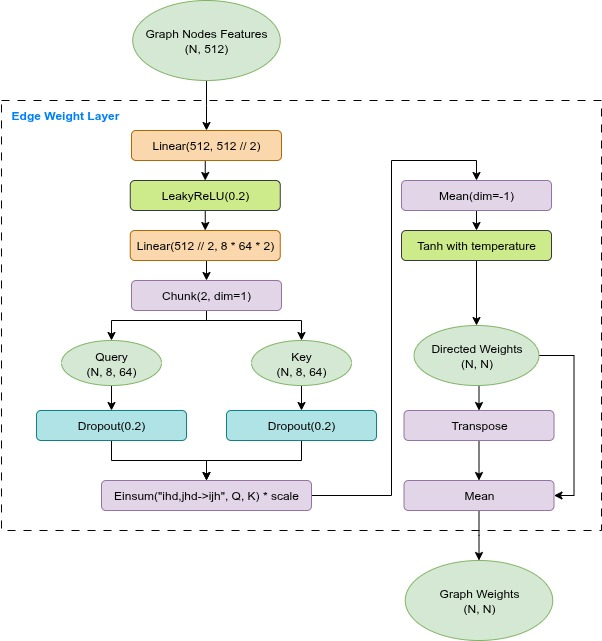
\includegraphics[width=0.8\linewidth]{images/part-02/chap-02/sec-01/EdgeWeightsLayer.jpg}
    \vspace{0.3cm}
    \caption{Kiến trúc của Edge Weights Layer sử dụng cơ chế Attention}
    \label{fig:KTEdgeWeightsLayer}
\end{figure}

\indent Mạng học trọng số cạnh được xây dựng dựa trên cơ chế \textit{self-attention}, trong đó tích vô hướng $Q \cdot K^{T}$ được sử dụng để thể hiện tính tương quan ngữ nghĩa giữa các nút \cite{vaswani2023attentionneed}. Đầu ra của tầng này sử dụng hàm kích hoạt \texttt{Tanh} nhằm giới hạn giá trị trọng số cạnh trong khoảng $[-1, 1]$, điều này cho phép mô hình biểu diễn hai loại quan hệ đối lập: quan hệ "bạn bè" với trọng số cạnh dương (tiệm cận 1) và quan hệ "đối kháng" với trọng số cạnh âm (tiệm cận $-1$).\vspace{0.3cm}

Việc cho phép tồn tại trọng số cạnh âm ở giai đoạn này đóng vai trò như một cơ chế lọc mềm. Với các giá trị trọng số âm sẽ được loại bỏ ở các tầng tiếp theo thông qua hàm \texttt{Clamp(min=0)}, nhờ đó mô hình có khả năng chủ động học cách loại bỏ các kết nối nhiễu hoặc không mang thông tin hữu ích. Phương pháp này linh hoạt hơn so với việc sử dụng hàm kích hoạt \texttt{Sigmoid}, vốn chỉ sinh ra các trọng số không âm trong khoảng $(0,1)$, điều này buộc mô hình phải duy trì tất cả các cạnh với mức độ ảnh hưởng khác nhau, kể cả những kết nối kém liên quan (có trọng số dương rất nhỏ, tiệm cận 0).\vspace{0.3cm}

Ngoài ra, để đảm bảo tính vô hướng của đồ thị, chỉ cần lấy ma trận trọng số cạnh tính được đem trung bình cộng với ma trận chuyển vị của chính nó. Cách xử lý này đảm bảo rằng trọng số liên kết giữa hai nút là nhất quán theo cả hai chiều, tức trọng số từ nút $A$ đến nút $B$ bằng với trọng số từ $B$ đến $A$.
